

\section{Đánh giá giải pháp}


\textit{Chương 5 của luận văn tập trung vào việc đánh giá và phân tích các giải pháp được đề xuất trong nghiên cứu. Mục tiêu chính của chương này là kiểm tra hiệu quả và tính khả thi của việc chuyển đổi từ MSSQL sang Greenplum trong việc quản lý cơ sở dữ liệu phân tán.}

\textit{Đầu tiên, chương này trình bày tổng quan về hệ thống phần mềm đã được xây dựng, bao gồm các thông tin chi tiết về số lượng dòng mã nguồn, số lượng hàm/lớp, và các mối liên hệ giữa chúng. Tiếp theo, chương này mô tả quy trình kiểm thử hệ thống, từ việc sử dụng các công cụ, thành phần và thư viện hỗ trợ cho đến các kết quả cụ thể thu được từ quá trình kiểm thử.}

\textit{Ngoài ra, chương này cũng phân tích những tính năng nổi bật của hệ thống phần mềm, nhấn mạnh các vấn đề thực tế mà giải pháp này đã giải quyết. Để đánh giá hiệu quả của giải pháp, chương 5 tiến hành so sánh các nghiệp vụ chính của hệ thống với một hệ thống tương tự, và sử dụng các độ đo tiêu chuẩn để đánh giá định lượng về lợi ích của giải pháp khi áp dụng vào môi trường thực tế.}

\textit{Cuối cùng, chương này kết luận về mức độ hoàn thành của các nhiệm vụ đề ra, đồng thời mở ra hướng phát triển và cải tiến trong tương lai cho hệ thống phần mềm.}


\subsection{Tổng quan về hệ thống} 

Hệ thống chuyển đổi từ MSSQL sang Greenplum, bao gồm những việc di chuyển dữ liệu, điều chỉnh lược đồ cơ sở dữ liệu và tích hợp vào hệ thống mới. Cơ sở dữ liệu mới không chỉ xử lý hiệu quả lượng dữ liệu lớn hơn mà còn cải thiện đáng kể hiệu suất truy vấn, đáp ứng nhu cầu ngày càng phức tạp của các hoạt động xử lý dữ liệu.


\subsection{Cải tiến và giải pháp}

Việc chuyển đổi hệ thống cơ sở dữ liệu từ MSSQL sang Greenplum đòi hỏi sự chuẩn bị kỹ lưỡng để đảm bảo dữ liệu và các chức năng ứng dụng không bị gián đoạn. Một trong những thách thức lớn trong quá trình này là việc xử lý mã hóa mật khẩu (hashing) do cách triển khai các hàm băm (hash functions) có thể khác nhau giữa hai hệ thống. Để giải quyết vấn đề này, cần viết lại mã để đảm bảo tính nhất quán trong việc mã hóa mật khẩu giữa MSSQL và Greenplum. Dưới đây là phân tích và giải pháp cho vấn đề này.

\subsection{Kiểm thử}


\begin{figure}
    \centering
    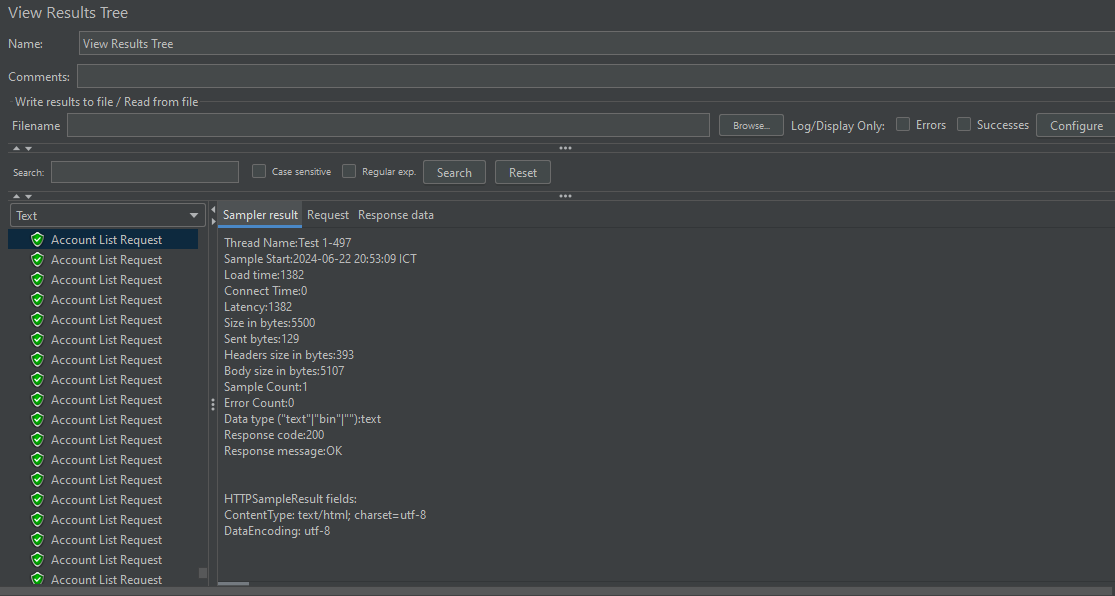
\includegraphics[width=0.8\linewidth]{vrt.png}
    \caption{View Results Tree trong JMeter}
    \label{fig:vrt}
\end{figure}

\begin{figure}
    \centering
    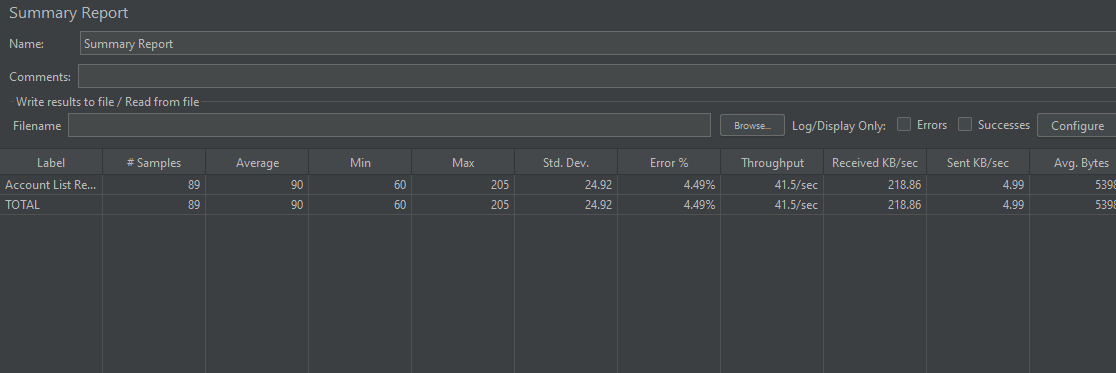
\includegraphics[width=0.8\linewidth]{sr.png}
     \caption{Summary Report trong JMeter}
    \label{fig:sr}
\end{figure}

\begin{figure}
    \centering
    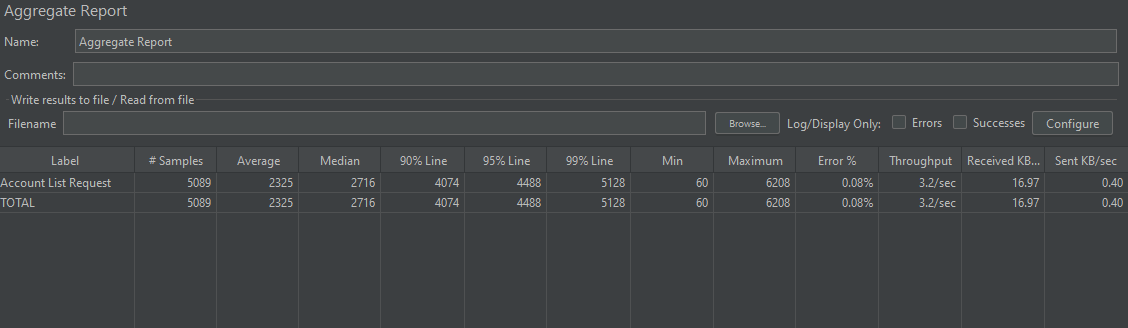
\includegraphics[width=0.8\linewidth]{ar.png}
    \caption{Aggregate Report trong JMeter}
    \label{fig:ar}
\end{figure}




Để thực hiện kiểm thử hiệu suất sử dụng Apache JMeter. Đầu tiên, truy cập trang chủ Apache JMeter\footnote{\url{https://jmeter.apache.org/download_jmeter.cgi}} và tải phiên bản mới nhất dưới dạng file ZIP hoặc TGZ. Sau khi giải nén file tải về vào một thư mục trên máy tính, cần cài đặt Java Development Kit (JDK) từ trang chủ Oracle JDK, chạy file cài đặt và thiết lập biến môi trường JAVA\_HOME trỏ tới thư mục cài đặt JDK, ví dụ: \verb|C:\Program Files\Java\jdk-11|. Chạy file jmeter.bat (trên Windows) hoặc jmeter (trên Unix/Linux) để khởi động giao diện người dùng của JMeter.


Trong JMeter, Thread Group là thành phần cốt lõi, nơi xác định số lượng người dùng ảo (threads) sẽ tương tác đồng thời với hệ thống. Để thêm Thread Group, chọn Add > Threads (Users) > Thread Group.

Listeners trong JMeter đóng vai trò quan trọng trong việc theo dõi, ghi nhận và trực quan hóa kết quả kiểm thử. Để thêm Listener vào Thread Group, chọn Add > Listener > Summary Report, Aggregate Report, View Results Tree như minh họa trong hình \ref{fig:testjmeter}.

Việc chuyển đổi dữ liệu từ MSSQL sang Greenplum đòi hỏi một bước kiểm định hiệu suất quan trọng để đảm bảo hệ thống mới vận hành mượt mà và đáp ứng mọi yêu cầu hiệu suất. Apache JMeter để tiến hành các bài kiểm thử toàn diện, đánh giá khả năng xử lý tải cao, độ tin cậy, và khả năng mở rộng của hệ thống.

JMeter đóng vai trò trung tâm trong quá trình kiểm thử, với Thread Group là thành phần cốt lõi. Thread Group cho phép xác định số lượng người dùng ảo (threads) tương tác đồng thời với Greenplum, mô phỏng các mức tải khác nhau, từ thấp đến cao, để đánh giá khả năng đáp ứng của hệ thống trong điều kiện thực tế.

Samplers trong JMeter, như HTTP Request Sampler, được sử dụng để gửi các yêu cầu (GET, POST) đến các điểm cuối cụ thể của Greenplum, mô phỏng hành vi người dùng thực. JMeter sẽ ghi lại kết quả trả về từ Greenplum để phân tích và đánh giá.

Trong quá trình đánh giá hiệu suất của hệ thống, nhiều độ đo quan trọng đã được áp dụng nhằm cung cấp cái nhìn toàn diện về khả năng xử lý và độ tin cậy của hệ thống trên hai nền tảng MSSQL và Greenplum. Thời gian trung bình (Average) được tính bằng cách chia tổng thời gian thực hiện tất cả các mẫu thử cho số lượng mẫu, giúp xác định tốc độ trung bình của hệ thống khi thực hiện các tác vụ. Trung vị (Median), đại diện cho giá trị giữa của tập hợp dữ liệu khi được sắp xếp theo thứ tự tăng dần, phản ánh hiệu suất thực tế của hệ thống mà không bị ảnh hưởng bởi các giá trị ngoại lệ. Các chỉ số phân vị (percentiles) như 90\%, 95\%, và 99\% cung cấp thông tin chi tiết về thời gian phản hồi trong các trường hợp ngoại lệ, nơi độ trễ có thể xảy ra. Thời gian nhỏ nhất và lớn nhất (Min, Max) đo lường khoảng thời gian nhanh nhất và chậm nhất mà hệ thống cần để hoàn thành một tác vụ, qua đó xác định các điểm cực đoan về hiệu suất. Cuối cùng, tỷ lệ lỗi (Error rate), biểu thị phần trăm các mẫu thử không thành công, là một chỉ số quan trọng để đánh giá độ tin cậy và ổn định của hệ thống khi phải đối mặt với khối lượng công việc lớn và các yêu cầu phức tạp. Những độ đo này không chỉ cung cấp thông tin chi tiết về hiệu suất mà còn giúp so sánh hiệu quả giữa hai nền tảng trong việc xử lý khối lượng dữ liệu lớn.

Listeners trong JMeter đóng vai trò quan trọng trong việc giám sát, ghi nhận và trực quan hóa kết quả kiểm thử. View Results Tree như hình \ref{fig:vrt} cung cấp chi tiết từng yêu cầu và phản hồi, giúp xác định các vấn đề cụ thể. Summary Report như hình \ref{fig:sr} tổng hợp thông tin hiệu suất hệ thống, bao gồm thời gian phản hồi trung bình, độ lệch chuẩn, và tỷ lệ yêu cầu thành công/thất bại. Aggregate Report như hình \ref{fig:ar} cung cấp dạng bảng tổng hợp các số liệu thống kê quan trọng như trung bình, trung vị, min, max, và phân vị 90\%, 95\%, 99\% của thời gian phản hồi. Các listener này cung cấp cái nhìn toàn diện về hoạt động của Greenplum dưới áp lực tải, từ đó đưa ra các điều chỉnh và tối ưu hóa cần thiết.



\subsection{Phân tích so sánh}

Luận văn này tập trung vào việc thiết kế, triển khai và đánh giá hiệu suất của một hệ thống phần mềm quản lý dữ liệu người dùng, được xây dựng trên hai nền tảng cơ sở dữ liệu phổ biến là MSSQL và Greenplum. Mục tiêu chính là so sánh và đánh giá hiệu quả của từng nền tảng trong việc xử lý khối lượng dữ liệu lớn, qua đó cung cấp cái nhìn sâu sắc về khả năng đáp ứng của từng hệ thống trong môi trường thực tế.

Cấu trúc dữ liệu của hệ thống được tổ chức thành năm bảng chính: aspnet\_Membership, aspnet\_Profile, aspnet\_Users, aspnet\_Roles, và aspnet\_UsersInRoles. Trong đó, các bảng aspnet\_Membership, aspnet\_Profile, aspnet\_Users, và aspnet\_UsersInRoles chứa 500.000 bản ghi mỗi bảng, trong khi bảng aspnet\_Roles chỉ có 2 bản ghi. Tổng khối lượng dữ liệu lên tới hơn 2 triệu bản ghi, tạo ra một thách thức đáng kể về hiệu suất xử lý, đặc biệt đối với các tác vụ quan trọng và thường xuyên như tìm kiếm, đăng ký, đăng nhập, và quản lý danh sách hồ sơ người dùng. Việc xử lý hiệu quả những tác vụ này đòi hỏi hệ thống không chỉ cần có khả năng tối ưu hóa cao mà còn phải phân phối tài nguyên một cách hiệu quả để đảm bảo đáp ứng nhanh chóng và chính xác các yêu cầu của người dùng.

\begin{table}[htbp]
\centering
\renewcommand{\arraystretch}{1.3} % Tăng khoảng cách giữa các hàng
\begin{tabular}{|l|c|c|c|}
\hline
\textbf{Tác vụ} & \textbf{Number of Threads (users)} & \textbf{Ramp-up period (seconds)} & \textbf{Loop Count} \\ \hline
\textbf{Tìm kiếm} & 40 & 2 & 5 \\ \hline
\textbf{Danh sách} & 30 & 5 & 5 \\ \hline
\textbf{Đăng ký} & 60 & 2 & 5 \\ \hline
\textbf{Đăng nhập} & 55 & 2 & 5 \\ \hline
\end{tabular}
\caption{Cấu hình kiểm thử cho các tác vụ}
\label{tab:task_configuration}
\end{table}

Bảng \ref{tab:task_configuration} trình bày các cấu hình kiểm thử được sử dụng trong quá trình thực hiện luận văn. Các cấu hình này bao gồm thông tin về số lượng người dùng mô phỏng (threads), thời gian để tất cả người dùng bắt đầu chạy (ramp-up period), và số lần lặp lại mỗi tác vụ (loop count). Các giá trị này được thiết lập dựa trên mục tiêu kiểm thử hệ thống hoạt có thể hoạt động khi bị chịu tải cao.




\subsubsection{So sánh Greenplum với MSSQL}

Để so sánh khả năng xử lý giữa hai hệ thống, MSSQL được triển khai trên một máy chủ với cấu hình gồm 4 vCPUs, 8GB RAM, và 160GB SSD. Trong khi đó, Greenplum được cài đặt trên ba máy chủ, mỗi máy trang bị 2 CPUs, 4GB RAM, và 80GB SSD, tổng hợp lại đạt 6 CPUs, 12GB RAM, và 240GB SSD. Sự khác biệt trong việc phân bổ tài nguyên và cấu hình phần cứng giữa hai hệ thống này tạo điều kiện cho việc đánh giá toàn diện về hiệu suất và khả năng mở rộng. Qua đó, xác định liệu Greenplum có phải là lựa chọn phù hợp hơn trong việc xử lý các tác vụ đòi hỏi hiệu suất cao trong môi trường dữ liệu lớn hay không.



\begin{table}[htbp]
\centering
\renewcommand{\arraystretch}{1.2}
\setlength{\tabcolsep}{4pt} 
\begin{tabular}{|l|c|c|c|c|c|c|c|c|c|}
\hline
\textbf{Hệ thống} & \textbf{\# Samples} & \textbf{Average} & \textbf{Median} & \textbf{90\% Line} & \textbf{95\% Line} & \textbf{99\% Line} & \textbf{Min} & \textbf{Max} & \textbf{Error \%} \\ \hline
MSSQL & 200 & 31,588 & 30,361 & 42,202 & 48,916 & 51,892 & 4,498 & 53,286 & 74.00\% \\ \hline
Greenplum & 200 & 26,028 & 26,933 & 28,756 & 35,264 & 43,497 & 8,966 & 44,382 & 0.00\% \\ \hline
\end{tabular}
\caption{So sánh hiệu suất giữa MSSQL và Greenplum cho tác vụ dăng ký tìm kiếm}
\label{tab:performance_comparison}
\end{table}

\begin{table}[htbp]
\centering
\renewcommand{\arraystretch}{1.2} % Tăng chiều cao của hàng để cải thiện khoảng cách
\setlength{\tabcolsep}{3.2pt} % Điều chỉnh khoảng cách giữa các cột
\begin{tabular}{|l|c|c|c|c|c|c|c|c|c|}
\hline
\textbf{Hệ thống} & \textbf{\# Samples} & \textbf{Average} & \textbf{Median} & \textbf{90\% Line} & \textbf{95\% Line} & \textbf{99\% Line} & \textbf{Min} & \textbf{Max} & \textbf{Error \%} \\ \hline
MSSQL & 150 & 281,862 & 241,553 & 607,490 & 628,493 & 633,736 & 32,274 & 709,878 & 28.00\% \\ \hline
Greenplum & 150 & 215,962 & 215,770 & 220,532 & 220,893 & 221,984 & 208,863 & 222,005 & 0.00\% \\ \hline
\end{tabular}
\caption{So sánh hiệu suất giữa MSSQL và Greenplum cho tác vụ danh sách}
\label{tab:performance_comparison_list}
\end{table}


\begin{table}[htbp]
\centering
\renewcommand{\arraystretch}{1.2} % Tăng chiều cao của hàng để cải thiện khoảng cách
\setlength{\tabcolsep}{4pt} % Điều chỉnh khoảng cách giữa các cột
\begin{tabular}{|l|c|c|c|c|c|c|c|c|c|}
\hline
\textbf{Hệ thống} & \textbf{\# Samples} & \textbf{Average} & \textbf{Median} & \textbf{90\% Line} & \textbf{95\% Line} & \textbf{99\% Line} & \textbf{Min} & \textbf{Max} & \textbf{Error \%} \\ \hline
MSSQL & 300 & 11,825 & 9,176 & 23,408 & 31,336 & 38,389 & 204 & 48,682 & 89.00\% \\ \hline
Greenplum & 300 & 51,755 & 53,409 & 66,165 & 72,707 & 75,179 & 131 & 76,786 & 0.00\% \\ \hline
\end{tabular}
\caption{So sánh hiệu suất giữa MSSQL và Greenplum cho tác vụ đăng ký}
\label{tab:performance_comparison_registration}
\end{table}

\begin{table}[htbp]
\centering
\renewcommand{\arraystretch}{1.2} % Tăng chiều cao của hàng để cải thiện khoảng cách
\setlength{\tabcolsep}{3.9pt} % Điều chỉnh khoảng cách giữa các cột
\begin{tabular}{|l|c|c|c|c|c|c|c|c|c|}
\hline
\textbf{Hệ thống} & \textbf{\# Samples} & \textbf{Average} & \textbf{Median} & \textbf{90\% Line} & \textbf{95\% Line} & \textbf{99\% Line} & \textbf{Min} & \textbf{Max} & \textbf{Error \%} \\ \hline
MSSQL & 275 & 25,149 & 25,327 & 39,150 & 40,701 & 44,437 & 1,134 & 47,866 & 11.64\% \\ \hline
Greenplum & 275 & 30,072 & 29,521 & 40,957 & 47,385 & 58,155 & 2,342 & 60,733 & 0.00\% \\ \hline
\end{tabular}
\caption{So sánh hiệu suất giữa MSSQL và Greenplum cho tác vụ đăng nhập}
\label{tab:performance_comparison_login}
\end{table}


Bảng \ref{tab:performance_comparison} thể hiện kết quả thực hiện tác vụ tìm kiếm, MSSQL thể hiện sự thiếu ổn định rõ rệt khi đối mặt với 40 người dùng đồng thời. Thời gian trung bình để hoàn thành một truy vấn tìm kiếm là 31,588 ms, với thời gian trung vị là 30,361 ms, cho thấy rằng một nửa số truy vấn mất ít nhất 30,361 ms để hoàn thành. Đáng chú ý là tỷ lệ lỗi lên tới 74\%, phản ánh rằng hệ thống gặp khó khăn lớn trong việc duy trì hiệu suất khi tải tăng cao. Các đường phân vị 90\%, 95\%, và 99\% lần lượt là 42,202 ms, 48,916 ms, và 51,892 ms, chỉ ra rằng ngay cả trong những điều kiện lý tưởng, MSSQL vẫn gặp phải các vấn đề về hiệu suất. Trong khi đó, Greenplum thể hiện sự ổn định và hiệu quả rõ rệt với cùng điều kiện kiểm thử. Hệ thống hoàn thành các truy vấn tìm kiếm với thời gian trung bình là 26,028 ms, và thời gian trung vị là 26,933 ms, phản ánh khả năng xử lý nhanh chóng và đồng nhất. Đặc biệt, Greenplum không ghi nhận bất kỳ lỗi nào trong suốt quá trình kiểm thử, cho thấy khả năng quản lý tài nguyên hiệu quả và xử lý đồng thời nhiều truy vấn mà không gặp vấn đề. Các đường phân vị 90\%, 95\%, và 99\% lần lượt là 28,756 ms, 35,264 ms, và 43,497 ms, khẳng định rằng Greenplum không chỉ xử lý các truy vấn nhanh chóng mà còn duy trì được hiệu suất cao ngay cả trong điều kiện tải nặng.

Bảng \ref{tab:performance_comparison_list} thể hiện kế quả thực hiện tác vụ xử lý danh sách, MSSQL gặp khó khăn khi phải đối mặt với 30 người dùng đồng thời. Thời gian trung bình để hoàn thành một truy vấn danh sách là 281,862 ms, với thời gian trung vị là 241,553 ms. Điều này cho thấy hệ thống cần một khoảng thời gian dài để xử lý các truy vấn, và hiệu suất giảm sút mạnh khi gặp phải lượng truy vấn lớn. Các giá trị của các đường phân vị 90\%, 95\%, và 99\% lần lượt là 607,490 ms, 628,493 ms, và 633,736 ms, phản ánh rằng hệ thống trở nên chậm chạp khi tải tăng cao. Thời gian thực hiện các truy vấn dao động từ 32,274 ms (Min) đến 709,878 ms (Max), thể hiện sự thiếu ổn định trong hiệu suất. Hơn nữa, tỷ lệ lỗi của MSSQL là 28\%, cho thấy hệ thống không thể duy trì hiệu suất khi phải xử lý lượng lớn truy vấn danh sách. Ngược lại, Greenplum cho thấy sự vượt trội trong việc duy trì hiệu suất ổn định với thời gian trung bình là 215,962 ms và thời gian trung vị là 215,770 ms, thấp hơn đáng kể so với MSSQL. Các giá trị của các đường phân vị 90\%, 95\%, và 99\% lần lượt là 220,532 ms, 220,893 ms, và 221,984 ms, minh chứng cho khả năng duy trì hiệu suất cao của Greenplum dù tải tăng. Thời gian thực hiện các truy vấn dao động từ 208,863 ms (Min) đến 222,005 ms (Max), cho thấy khả năng xử lý đồng đều và ổn định trong các điều kiện khác nhau. Đặc biệt, Greenplum không gặp phải bất kỳ lỗi nào, thể hiện khả năng quản lý và xử lý hiệu quả các tác vụ danh sách.

Bảng \ref{tab:performance_comparison_registration} thể hiện kế quả thực hiện   tác vụ đăng ký, MSSQL tiếp tục bộc lộ những hạn chế trong việc xử lý đồng thời với thời gian trung bình là 11,825 ms và thời gian trung vị là 9,176 ms. Các đường phân vị 90\%, 95\%, và 99\% lần lượt là 23,408 ms, 31,336 ms, và 38,389 ms, cho thấy rằng hệ thống gặp phải sự chậm trễ đáng kể khi phải xử lý các truy vấn phức tạp. Đáng lo ngại là tỷ lệ lỗi lên tới 89\%, chỉ ra rằng MSSQL không thể đáp ứng được lượng yêu cầu đăng ký đồng thời lớn. Thời gian thực hiện các truy vấn dao động từ 204 ms (Min) đến 48,682 ms (Max), phản ánh sự thiếu ổn định trong hiệu suất của hệ thống. Tuy thời gian trung bình của Greenplum trong tác vụ đăng ký là 51,755 ms, cao hơn so với MSSQL, nhưng hệ thống này lại không gặp phải bất kỳ lỗi nào. Thời gian trung vị là 53,409 ms, và các đường phân vị 90\%, 95\%, và 99\% lần lượt là 66,165 ms, 72,707 ms, và 75,179 ms, chứng tỏ Greenplum có khả năng duy trì hiệu suất chấp nhận được ngay cả khi tải tăng cao. Thời gian thực hiện các truy vấn dao động từ 131 ms (Min) đến 76,786 ms (Max), cho thấy khả năng xử lý ổn định của hệ thống ngay cả trong điều kiện tải nặng.

Bảng \ref{tab:performance_comparison_login} thể hiện kế quả thực hiện  tác vụ đăng nhập, MSSQL và Greenplum tiếp tục thể hiện sự khác biệt đáng kể về hiệu suất. MSSQL có thời gian trung bình là 25,149 ms và thời gian trung vị là 25,327 ms, với các đường phân vị 90\%, 95\%, và 99\% lần lượt là 39,150 ms, 40,701 ms, và 44,437 ms. Dù thời gian thực hiện các truy vấn dao động từ 1,134 ms (Min) đến 47,866 ms (Max), tỷ lệ lỗi của MSSQL vẫn là 11.64\%, cho thấy hệ thống gặp khó khăn trong việc duy trì hiệu suất ổn định dưới áp lực từ nhiều người dùng đồng thời. Greenplum mặc dù có thời gian trung bình là 30,072 ms và thời gian trung vị là 29,521 ms, vẫn duy trì được sự ổn định vượt trội. Các đường phân vị 90\%, 95\%, và 99\% lần lượt là 40,957 ms, 47,385 ms, và 58,155 ms, cho thấy rằng Greenplum tuy có chậm hơn một chút so với MSSQL trong một số trường hợp, nhưng không có lỗi nào được ghi nhận. Điều này khẳng định rằng Greenplum có khả năng quản lý tài nguyên tốt hơn và xử lý hiệu quả các yêu cầu đăng nhập đồng thời, đảm bảo hiệu suất cao và ổn định.


\subsubsection{Khả năng mở rộng của Greenplum}

Để đánh giá khả năng mở rộng của hệ thống cơ sở dữ liệu Greenplum, số lượng segment đã được tăng từ 3 node lên 6 node, với mỗi node được duy trì cấu hình ban đầu gồm 2 CPUs, 4GB RAM, và 80GB SSD. Việc mở rộng này nâng tổng tài nguyên của hệ thống lên 12 CPUs, 24GB RAM, và 480GB SSD, nhằm mục tiêu kiểm tra tác động của việc nhân đôi số lượng node theo chiều ngang đến hiệu suất tổng thể của hệ thống. Việc tăng số lượng node không chỉ đơn thuần là thêm tài nguyên phần cứng, mà còn là phép thử về cách hệ thống phân phối tải, tối ưu hóa quá trình xử lý, và duy trì hiệu suất ổn định trong điều kiện tải cao hơn. Qua đó, thử nghiệm này cung cấp những hiểu biết sâu sắc về khả năng mở rộng và hiệu quả của Greenplum trong môi trường thực tế yêu cầu xử lý dữ liệu lớn và đồng thời nhiều người dùng.

\begin{table}[htbp]
\centering
\renewcommand{\arraystretch}{1.2} % Tăng chiều cao của hàng để cải thiện khoảng cách
\setlength{\tabcolsep}{2pt} % Điều chỉnh khoảng cách giữa các cột
\begin{tabular}{|l|c|c|c|c|c|c|c|c|c|}
\hline
\textbf{Hệ thống} & \textbf{\# Samples} & \textbf{Average} & \textbf{Median} & \textbf{90\% Line} & \textbf{95\% Line} & \textbf{99\% Line} & \textbf{Min} & \textbf{Max} & \textbf{Error \%} \\ \hline
Greenplum & 200 & 26,028 & 26,933 & 28,756 & 35,264 & 43,497 & 8,966 & 44,382 & 0.00\% \\ \hline
Greenplum mở rộng & 200 & 12,583 & 13,324 & 15,891 & 16,757 & 17,682 & 2,747 & 18,163 & 0.00\% \\ \hline
\end{tabular}
\caption{So sánh hiệu suất giữa Greenplum và Greenplum mở rộng cho tác vụ dăng ký tìm kiếm}
\label{tab:Greenplum_extended_comparison_search}
\end{table}

\begin{table}[htbp]
\centering
\renewcommand{\arraystretch}{1.2} % Tăng chiều cao của hàng để cải thiện khoảng cách
\setlength{\tabcolsep}{1.5pt} % Điều chỉnh khoảng cách giữa các cột
\begin{tabular}{|l|c|c|c|c|c|c|c|c|c|}
\hline
\textbf{Hệ thống} & \textbf{\# Samples} & \textbf{Average} & \textbf{Median} & \textbf{90\% Line} & \textbf{95\% Line} & \textbf{99\% Line} & \textbf{Min} & \textbf{Max} & \textbf{Error \%} \\ \hline
Greenplum & 150 & 215,962 & 215,770 & 220,532 & 220,893 & 221,984 & 208,863 & 222,005 & 0.00\% \\ \hline
Greenplum mở rộng & 150 & 117,429 & 117,520 & 123,688 & 126,481 & 134,354 & 98,074 & 136,692 & 0.00\% \\ \hline
\end{tabular}
\caption{So sánh hiệu suất giữa Greenplum và Greenplum mở rộng cho tác vụ danh sách}
\label{tab:Greenplum_extended_comparison_list}
\end{table}

\begin{table}[htbp]
\centering
\renewcommand{\arraystretch}{1.2} % Tăng chiều cao của hàng để cải thiện khoảng cách
\setlength{\tabcolsep}{2pt} % Điều chỉnh khoảng cách giữa các cột
\begin{tabular}{|l|c|c|c|c|c|c|c|c|c|}
\hline
\textbf{Hệ thống} & \textbf{\# Samples} & \textbf{Average} & \textbf{Median} & \textbf{90\% Line} & \textbf{95\% Line} & \textbf{99\% Line} & \textbf{Min} & \textbf{Max} & \textbf{Error \%} \\ \hline
Greenplum & 300 & 51,755 & 53,409 & 66,165 & 72,707 & 75,179 & 131 & 76,786 & 0.00\% \\ \hline
Greenplum mở rộng & 300 & 26,677 & 26,620 & 33,057 & 35,946 & 40,804 & 171 & 41,939 & 0.00\% \\ \hline
\end{tabular}
\caption{So sánh hiệu suất giữa Greenplum và Greenplum mở rộng cho tác vụ đăng ký}
\label{tab:Greenplum_extended_comparison_registation}
\end{table}

\begin{table}[htbp]
\centering
\renewcommand{\arraystretch}{1.2} % Tăng chiều cao của hàng để cải thiện khoảng cách
\setlength{\tabcolsep}{3.5pt} % Điều chỉnh khoảng cách giữa các cột
\begin{tabular}{|l|c|c|c|c|c|c|c|c|c|}
\hline
\textbf{Hệ thống} & \textbf{Samples} & \textbf{Average} & \textbf{Median} & \textbf{90\% Line} & \textbf{95\% Line} & \textbf{99\% Line} & \textbf{Min} & \textbf{Max} & \textbf{Error \%} \\ \hline
Greenplum & 275 & 30,072 & 29,521 & 40,957 & 47,385 & 58,155 & 2,342 & 60,733 & 0.00\% \\ \hline
Greenplum mở rộng & 275 & 16,906 & 17,336 & 23,216 & 25,823 & 29,972 & 1,504 & 35,425 & 0.00\% \\ \hline
\end{tabular}
\caption{So sánh hiệu suất giữa Greenplum và Greenplum mở rộng cho tác vụ đăng nhập}
\label{tab:Greenplum_extended_comparison_login}
\end{table}



Bảng \ref{tab:Greenplum_extended_comparison_search} cho thấy việc mở rộng hệ thống mang lại sự cải thiện đáng kể về hiệu suất. Thời gian xử lý trung bình của Greenplum giảm từ 26,028 ms xuống còn 12,583 ms, giảm gần 50\%. Thời gian trung vị cũng giảm tương ứng từ 26,933 ms xuống còn 13,324 ms. Các đường phân vị 90\%, 95\%, và 99\% (28,756 ms, 35,264 ms, và 43,497 ms) trong phiên bản ban đầu đều giảm xuống (15,891 ms, 16,757 ms, và 17,682 ms) trong phiên bản mở rộng, cho thấy rằng hệ thống mở rộng không chỉ nhanh hơn mà còn duy trì hiệu suất cao và ổn định hơn trong điều kiện tải lớn.

Bảng \ref{tab:Greenplum_extended_comparison_list} thể hiện kết quả thực hiện tác vụ danh sách. Hệ thống mở rộng tiếp tục thể hiện hiệu quả với thời gian xử lý trung bình giảm từ 215,962 ms xuống còn 117,429 ms. Thời gian trung vị cũng được cải thiện đáng kể, giảm từ 215,770 ms xuống còn 117,520 ms. Các đường phân vị 90\%, 95\%, và 99\% giảm từ 220,532 ms, 220,893 ms, và 221,984 ms xuống còn 123,688 ms, 126,481 ms, và 134,354 ms tương ứng, phản ánh sự cải thiện đáng kể về hiệu suất khi hệ thống phải xử lý các truy vấn phức tạp trên khối lượng dữ liệu lớn.

Bảng \ref{tab:Greenplum_extended_comparison_registation} thể hiện kết quả thực hiện tác vụ đăng ký. Việc mở rộng hệ thống đã giúp giảm thời gian trung bình từ 51,755 ms xuống còn 26,677 ms, trong khi thời gian trung vị giảm từ 53,409 ms xuống còn 26,620 ms. Các đường phân vị 90\%, 95\%, và 99\% cũng giảm từ 66,165 ms, 72,707 ms, và 75,179 ms xuống còn 33,057 ms, 35,946 ms, và 40,804 ms. Những kết quả này cho thấy rằng hệ thống mở rộng không chỉ tăng tốc độ xử lý mà còn duy trì tính ổn định, đặc biệt khi phải xử lý đồng thời số lượng lớn yêu cầu đăng ký từ nhiều người dùng.

Bảng \ref{tab:Greenplum_extended_comparison_login} thể hiện kết quả thực hiện tác vụ đăng nhập. Hệ thống Greenplum mở rộng cũng thể hiện sự vượt trội trong tác vụ đăng nhập, với thời gian trung bình giảm từ 30,072 ms xuống còn 16,906 ms, và thời gian trung vị giảm từ 29,521 ms xuống còn 17,336 ms. Các đường phân vị 90\%, 95\%, và 99\% giảm từ 40,957 ms, 47,385 ms, và 58,155 ms xuống còn 23,216 ms, 25,823 ms, và 29,972 ms. Thời gian xử lý tối thiểu và tối đa cũng giảm, cho thấy hệ thống không chỉ nhanh hơn mà còn ổn định hơn, giảm thiểu đáng kể thời gian thực hiện cho các truy vấn đăng nhập.



Từ kết quả phân tích, có thể kết luận rằng Greenplum có kết quả tốt hơn so với MSSQL trong việc xử lý các tác vụ dưới điều kiện tải cao. Greenplum không chỉ hoàn thành các tác vụ nhanh hơn trong nhiều trường hợp mà còn duy trì sự ổn định và độ tin cậy, đặc biệt với tỷ lệ lỗi bằng 0\% trong hầu hết các tác vụ. Điều này chứng tỏ rằng trong những môi trường yêu cầu cao về hiệu suất và khả năng xử lý song song, Greenplum là lựa chọn ưu việt hơn so với MSSQL, đặc biệt khi phải đối mặt với các khối lượng công việc lớn.

Kết quả nghiên cứu cũng khẳng định rằng việc mở rộng hệ thống Greenplum từ 3 node lên 6 node đã mang lại những cải thiện đáng kể về hiệu suất trong tất cả các tác vụ được kiểm thử. Thời gian xử lý giảm rõ rệt, đặc biệt trong các tác vụ đòi hỏi hiệu suất cao như xử lý danh sách và đăng ký. Các chỉ số phân vị cho thấy hệ thống mở rộng không chỉ nhanh hơn mà còn ổn định hơn, giúp giảm thiểu tối đa thời gian xử lý các truy vấn phức tạp và duy trì hiệu suất ổn định ngay cả khi số lượng người dùng tăng lên. Việc không ghi nhận bất kỳ lỗi nào trong cả hai phiên bản hệ thống càng nhấn mạnh tính ổn định và độ tin cậy của Greenplum. Những kết quả này cho thấy việc mở rộng số lượng node là một chiến lược hiệu quả để nâng cao khả năng xử lý và đảm bảo hiệu suất ổn định của Greenplum trong các môi trường dữ liệu lớn, đáp ứng tốt hơn các yêu cầu thực tiễn về quản lý và xử lý dữ liệu đồng thời.
